% Created by Bonita Graham
% Last update: February 2019 By Kestutis Bendinskas

% Authors: 
% Please do not make changes to the preamble until after the solid line of %s.

\documentclass[10pt]{article}
\usepackage[explicit]{titlesec}
\setlength{\parindent}{0pt}
\setlength{\parskip}{1em}
\usepackage{hyphenat}
\usepackage{ragged2e}
\RaggedRight

% These commands change the font. If you do not have Garamond on your computer, you will need to install it.
%\usepackage{garamondx}
\usepackage[T1]{fontenc}
\usepackage{amsmath, amsthm}
\usepackage{graphicx}
\usepackage{placeins}

% This adjusts the underline to be in keeping with word processors.
\usepackage{soul}
\setul{.6pt}{.4pt}


% The following sets margins to 1 in. on top and bottom and .75 in on left and right, and remove page numbers.
\usepackage{geometry}
\geometry{vmargin={1in,1in}, hmargin={.75in, .75in}}
\usepackage{fancyhdr}
\pagestyle{fancy}
\pagenumbering{gobble}
\renewcommand{\headrulewidth}{0.0pt}
\renewcommand{\footrulewidth}{0.0pt}

% These Commands create the label style for tables, figures and equations.
%\usepackage[labelfont={footnotesize,bf} , textfont=footnotesize]{caption}
\usepackage{caption}
\usepackage{subcaption}
\captionsetup{labelformat=simple, labelsep=period}
\newcommand\num{\addtocounter{equation}{1}\tag{\theequation}}
\renewcommand{\theequation}{\arabic{equation}}
\makeatletter
\renewcommand\tagform@[1]{\maketag@@@ {\ignorespaces {\footnotesize{\textbf{Equation}}} #1.\unskip \@@italiccorr }}
\makeatother
\setlength{\intextsep}{10pt}
\setlength{\abovecaptionskip}{0pt}
\setlength{\belowcaptionskip}{10pt}

\renewcommand{\textfraction}{0.10}
\renewcommand{\topfraction}{0.85}
\renewcommand{\bottomfraction}{0.85}
\renewcommand{\floatpagefraction}{0.90}

% These commands set the paragraph and line spacing
\titleformat{\section}
  {\normalfont}{\thesection}{1em}{\MakeUppercase{\textbf{#1}}}
\titlespacing\section{0pt}{0pt}{-10pt}
\titleformat{\subsection}
  {\normalfont}{\thesubsection}{1em}{\textit{#1}}
\titlespacing\subsection{0pt}{0pt}{-8pt}
\renewcommand{\baselinestretch}{1.15}

% This designs the title display style for the maketitle command
\makeatletter
\newcommand\sixteen{\@setfontsize\sixteen{16pt}{6}}
\renewcommand{\maketitle}{\bgroup\setlength{\parindent}{0pt}
\begin{flushleft}
\vspace{-.375in}
\sixteen\bfseries \@title
\medskip
\end{flushleft}
\textit{\@author}
\egroup}
\makeatother

% This styles the bibliography and citations.
%\usepackage[biblabel]{cite}
\usepackage[sort&compress]{natbib}
\setlength\bibindent{2em}
\makeatletter
\renewcommand\@biblabel[1]{\textbf{#1.}\hfill}
\makeatother
\renewcommand{\citenumfont}[1]{\textbf{#1}}
\bibpunct{}{}{,~}{s}{,}{,}
\setlength{\bibsep}{0pt plus 0.3ex}




%%%%%%%%%%%%%%%%%%%%%%%%%%%%%%%%%%%%%%%%%%%%%%%%%

% Authors: Add additional packages and new commands here.  
% Limit your use of new commands and special formatting.

% Place your title below. Use Title Capitalization.
\title{Pseudopotential (ECP) Development, Roadmap and Requests}

% Add author information below. Communicating author is indicated by an asterisk, the affiliation is shown by superscripted lower case letter if several affiliations need to be noted.
%\author{
%Jane Smith*$^{a}$, John Smith$^{b}$ \\ \medskip \bigskip
%$^{a}$Department of AA, BB University, City, ST (italicized, state is listed as a two-capital letter designation) \\ 
%$^{b}$Department of CC, DD University, City, ST (italicized, state is listed as a two-capital letter designation)\\ %\medskip \bigskip
%https://doi.org/10.33697/ajur.2019.003\\ \medskip \bigskip



\pagestyle{empty}
\begin{document}

% Makes the title and author information appear.
\vspace*{.01 in}
\maketitle
\vspace{.12 in}

% Abstracts are required.
\section*{abstract}
This document is intended to collect the current activities of the pseudopotential (ECP) development effort within the CMS, to collect ideas about what has been done, what is being worked on, pain points and requests for new potentials

% Keywords are required.
%\section*{keywords} 
%List Eight to Ten Capitalized Keywords Separated by \ul{Semicolons}; Do Not Use Period at The End

\vspace{.12 in}

% Start the main part of the manuscript here.
% Comment out section headings if inappropriate to your discipline.
% If you add additional section or subsection headings, use an asterisk * to avoid numbering. 

\section*{Current Status}
Current ECPs covering developed by NCSU cover the first three rows of the periodic table.  Papers concerning their construction are found \cite{first-ecps, second-ecps, third-row, update} in the literature.  They were constructed to have good transferrability and to be as iso-spectral as possible with all electron correlated calculations.  They are available at www.pseudopotentiallibrary.org.  They also include gaussian style basis sets for use in quantum chemistry style calculations.

There are a number of outstanding issues to address 
\begin{itemize}
    \item Projectors are available for most ECPs for use in Kleinman-Bylander plane wave DFT codes.  These may currently be hard and their transferrability is not guaranteed.
    \item The format for including spin-orbit terms as been defined, but currently there are no ECPs available that use this.
    \item Transferrability data is not readily available outside of papers for the ECPs, furthermore it is difficult to assess trade-offs when trying to look for something like a potential with a lower cutoff or smaller / more amenable basis set.
\end{itemize}


\section*{requests}
such and such is hard.
Please make element x for reason y



\section*{current work}
So and so is doing element x


\section{Iron}

I generated another softer ECP for Fe in the same scheme as ccECPs, labeled as ccECP-soft. The KE cutoff is about 700 Ry. Below is the atomic gaps and molecular transferability test. Original published ccECP is included there as comparison too.

The Fe ccECP-soft parameter is give below and can also be downloaded under ./ccECP-soft-param/ directory:\\
16 3  \\
2 2 4 \\
2 8.9890516 13.9428916  \\  
2 14.963588  189.50111  \\
2 9.9838449 25.8036121  \\
2 14.979791  95.801262  \\
1 12.000794  16.0  \\
3 9.9968683 192.012710  \\
2 9.4029511 -110.30045  \\
2 5.9990706 2.59183990  \\

\begin{figure*}[!htbp]
\centering
\begin{subfigure}{0.5\textwidth}
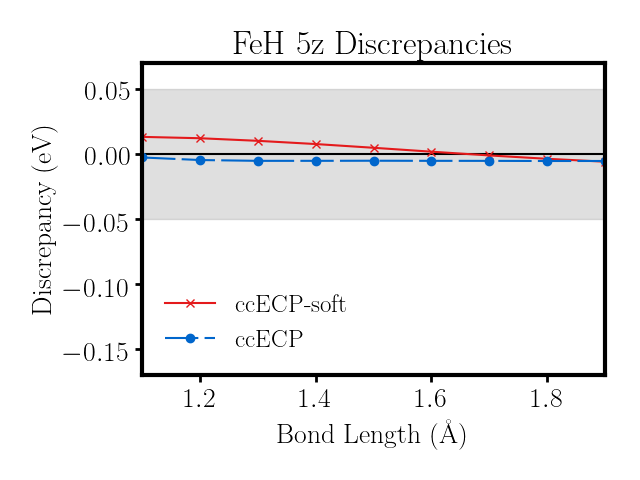
\includegraphics[width=\textwidth]{figures/FeH_5z.png}
\caption{FeH 5Z binding curve discrepancies}
\label{fig:FeO_5z}
\end{subfigure}%
\begin{subfigure}{0.5\textwidth}
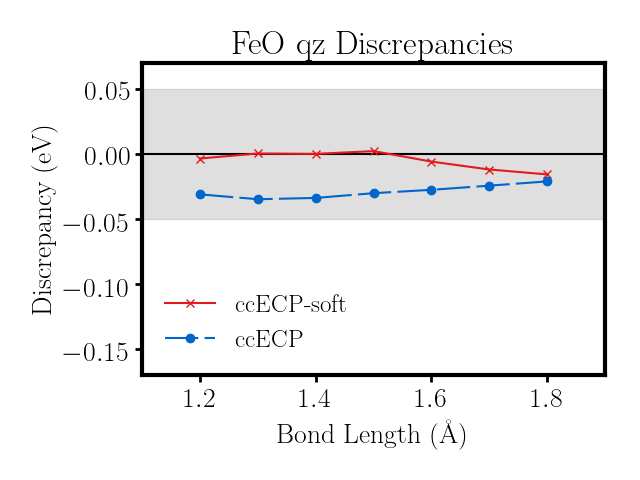
\includegraphics[width=\textwidth]{figures/FeO_qz.png}
\caption{FeO QZ binding curve discrepancies}
\label{fig:FeO_qz}
\end{subfigure}
\caption{Binding energy discrepancies for (a) FeH 5Z and (b) FeO QZ molecules with regard to CCSD(T). The shaded region indicates the band of chemical accuracy. The dashed vertical line represents the equilibrium geometry.}
\label{fig:Fe_mols}
\end{figure*}




\begin{table*}[!htbp]
\setlength{\tabcolsep}{3pt} %% default is 6pt
\centering
\caption{Fe gaps and relative errors for various ECPs.  All values in eV}
\resizebox{0.5\textwidth}{!}{%
\begin{tabular}{ll|cccccccccr}
\hline\hline
States and Symmetry &   &   AE &        ccECP   &   ccECP-soft  \\
\hline
{[Ar] $3d^74s^2$ } EA    & $^4F$ & -0.0579872 & -0.005436 &     -0.003053 \\
{[Ar] $3d^74s^1$ }       & $^5F$ &    0.88855 & -0.014150 &     -0.021149 \\
{[Ar] $3d^8$ }           & $^3F$ &    4.15711 & -0.017024 &     -0.019415 \\
{[Ar] $3d^64s^1$ }       & $^6D$ &    7.88583 & -0.016111 &     -0.034720 \\
{[Ar] $3d^7$ }           & $^4F$ &    8.16252 & -0.002125 &     -0.044298 \\
{[Ar] $3d^6$ }   2nd Ion & $^5D$ &    24.0909 &  0.013863 &     -0.041475 \\
{[Ar] $3d^5$ }   3rd Ion & $^5S$ &    54.6615 &  0.021912 &      0.005008 \\
\hline
MAD & &                                     &  0.012946 &      0.024160 \\
\hline
\hline
\end{tabular}
}
\end{table*}


\section{Cobalt}

 The KE cutoff of ccECP-soft Co is about 700 Ry. Below is the atomic gaps and molecular transferability test. Original published ccECP is included there as comparison too.

Note that here I have an ECP labeled as 600Ry, this is generated by Cody using Opium package from Troullier-Martins method fitting from original ccECPs. It is a numerical ECP but I fit it into Gaussian and test it in atomic gaps and molecules. The fit is not perfect and can not represent the full accuracy of it.

The Co ccECP-soft parameter is give below and can also be downloaded under ./ccECP-soft-param/ directory:\\
17 3  \\
2 2 4 \\
2 10.013765  15.836729    \\ 
2 15.026211  172.58644    \\
2 7.9885909 15.3494954    \\
2 14.997586  90.995647    \\
1 12.003882  17.0    \\
3 10.005064  204.06599    \\
2 9.4548033 -117.74448    \\
2 6.0069244 2.85018517    \\


\begin{figure*}[!htbp]
\centering
\begin{subfigure}{0.5\textwidth}
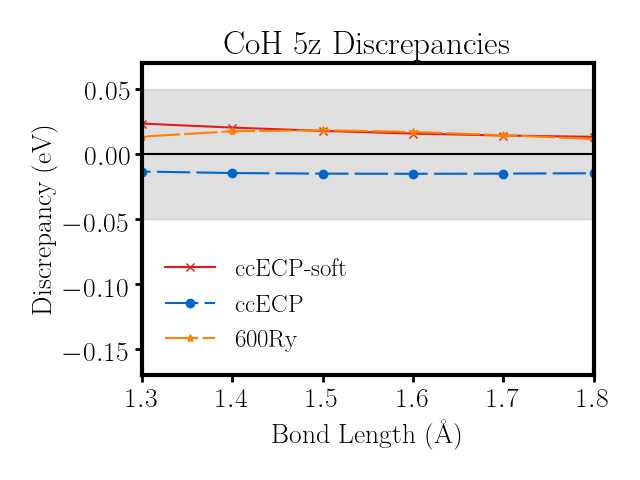
\includegraphics[width=\textwidth]{figures/CoH_5z.png}
\caption{CoH 5Z binding curve discrepancies}
\label{fig:CoO_5z}
\end{subfigure}%
\begin{subfigure}{0.5\textwidth}
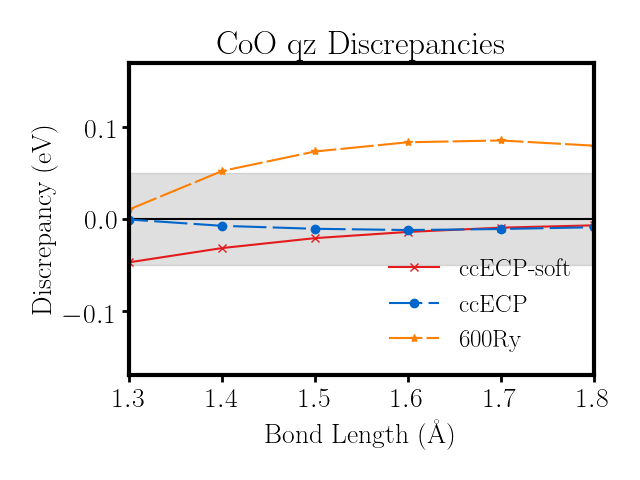
\includegraphics[width=\textwidth]{figures/CoO_qz.png}
\caption{CoO QZ binding curve discrepancies}
\label{fig:CoO_qz}
\end{subfigure}
\caption{Binding energy discrepancies for (a) CoH 5Z and (b) CoO QZ molecules with regard to CCSD(T). The shaded region indicates the band of chemical accuracy. }%The dashed vertical line represents the equilibrium geometry.}
\label{fig:Co_mols}
\end{figure*}



\begin{table*}[!htbp]
\setlength{\tabcolsep}{3pt} %% default is 6pt
\centering
\caption{Co gaps and relative errors for various ECPs.  All values in eV}
\resizebox{0.5\textwidth}{!}{%
\begin{tabular}{ll|cccccccccr}
\hline\hline
States and Symmetry &   &   AE &        ccECP   &   ccECP-soft   &  600Ry  \\
\hline
{[Ar] $3d^84s^2$ }    EA  & $^3F$ & -0.648825 & -0.011727 &   0.023771 &  0.017302  \\
{[Ar] $3d^84s^1$ }        & $^4F$ &  0.404998 & -0.018725 &   0.010404 & -0.022794  \\
{[Ar] $3d^9$ }            & $^2D$ &   3.29022 & -0.028436 &   0.018581 &  0.053097  \\
{[Ar] $3d^74s^1$ }        & $^5F$ &    8.2851 & -0.014988 &  -0.025523 & -0.006439  \\
{[Ar] $3d^8$ }            & $^3F$ &   7.85217 & -0.013046 &  -0.004582 & -0.038360  \\
{[Ar] $3d^7$ }  2nd Ion   & $^4F$ &   24.9596 &  0.005217 &  -0.024421 &  0.062209  \\
{[Ar] $3d^6$ }  3rd Ion   & $^5D$ &   58.4749 &  0.009923 &  -0.040255 &  0.461901  \\
\hline
MAD & &                                     &  0.014580 &   0.021077   &  0.094586  \\
\hline
\hline
\end{tabular}
}
\end{table*}

\end{document}
